\chapter{Diskussion}

\section{Einsatz der Objektdetektoren in der Industrie}

Die Bewertung der beiden Detektoren für den industriellen Einsatz baut auf den in Kapitel \ref{eval} eingeführten Bewertungskriterien auf. 

Hinsichtlich der Präzision fallen beide Objektdetektoren besser als die ursprünglichen Referenzergebnisse aus den wissenschaftlichen Veröffentlichungen aus. Es ist aber zu bemerken, dass die Ergebnisse nicht gut mit denen der wissenschaftlichen Veröffentlichungen vergleichbar sind, da sie auf unterschiedlichen, deutlich einfacheren Daten trainiert wurden. Der Vergleichsdatensatz ist hierbei \textit{PascalVOC 2007}, der 20 Klassen besitzt und damit für das Modell komplexer zu modellieren ist, als der \textit{SmartWarehouse} Datensatz mit nur 9 Klassen. Mit 83,1\% fällt \textit{SSD300} um 8,8\% besser aus, während \textit{YOLOv3} sogar eine Verbesserung von 16.7\% verzeichnet. Dennoch lässt sich darauf schließen, dass beide Implementierungen bezüglich Präzision in einer Größenordnung skalieren, die dem Niveau der Vergleichsergebnisse aus \textit{PascalVOC 2007} nachkommt. Die leicht erhöhte Präzision von \textit{SSD300} gegenüber \textit{YOLOv3} liegt daran, dass \textit{SSD300} im Gegensatz zu \textit{YOLOv3} Bounding Box Vorschläge unterschiedlicher Seitenverhältnisse zulässt und die Unterteilung in Gitterstrukturen ebenfalls für mehrere Skalierungen durchgeführt wird. Dies wird vor allem erkenntlich beim Vergleich der \textit{mAP} bei den Klassen \textit{Pepsi Cola Groß} und \textit{Pepsi Cola Klein}. Objekte der Klassen sehen grundsätzlich gleich aus, nur die Größe ändert sich, sind also unterschiedlich skaliert. Lässt man den Effekt bei unterschiedlichen Skalierungen allerdings außer Auge, so schneidet \textit{YOLOv3} dennoch besser ab als \textit{SSD300} auf Basis des \textit{SmartWarehouse} Datensatzes (siehe Tabelle \ref{table:yoloresults}).

Ein weiteres Bewertungskriterium ist das Reaktionsvermögen. Hier schneidet \textit{SSD300} mit durchschnittlich 31 FPS leicht besser ab als \textit{YOLOv3} mit 28 FPS, wobei dieser Unterschied kaum als wahres Entscheidungskriterium gesehen werden sollte, \textit{SSD300} \textit{YOLOv3} vorzuziehen. Auf einem leichten Datensatz wie \textit{SmartWarehouse} gibt es also kaum Unterschiede im Reaktionsvermögen als im Vergleich zu größeren und komplexeren Datensätzen wie \textit{PascalVOC 2007} (siehe Abbildung \ref{result}). Laut wissenschaftlichen Referenzergebnissen scheidet hier \textit{SSD300} um 25 FPS besser ab als \textit{YOLO}.

Bezüglich Trainingsverhalten könnte \textit{SSD300} das Training mit leistungsfähigeren Grafikkarten wie der \textit{NVIDIA Tesla V100} von 16,5 Stunden auf umgerechnet 5,2 Stunden geschätzt rund drei Mal schneller vollziehen. Die Rechnung legt die Tabelle \ref{table:comparison} zugrunde. Pro Sekunde kann eine \textit{NVIDIA GeForce GTX 1080} hierbei $2560\cdot 9,784 = 25.047,04 TeraFLOPs$ vollziehen im Vergleich zu $5120\cdot 14,13 = 72.345,6 TeraFLOPs$ pro Sekunde bei einer \textit{NVIDIA Tesla V100}. Da die \textit{NVIDIA Tesla V100} zusätzlich noch über Tensor Cores verfügt, kann der Zeitgewinn sogar noch höher eingeschätzt werden. Bei acht \textit{NVIDIA Tesla V100} betragen die Trainingskosten so beispielsweise nur noch ca. 39 Minuten. Somit lässt sich festhalten, dass sich \textit{SSD300} durchaus mit aktuellen Cloud Grafikkarten effizient trainieren lassen lässt. Da die Custom-Implementierung allerdings Hilfsstrukturen auf dem Sekundärspeicher erstellt, können hierbei beim Trainieren auf der Cloud Probleme auftreten. Meistens wird der Sekundärspeicher auf virtuellen Maschinen in der Cloud zum Schutz vor Angriffen nur \textit{read-only} bereitgestellt. 

\textit{YOLOv3} ließ sich mit acht Stunden deutlich schneller trainieren, allerdings unter vollkommen anderen Voraussetzungen. Nicht nur die verwendeten \textit{Deep Learning} Frameworks sind unterschiedlich, sondern auch die Trainingshardware. Als Grafikkarte wurde bei \textit{YOLOv3} eine \textit{NVIDIA GeForce RTX 2060 SUPER} verwendet, die zusätzlich über 272 Tensor Cores verfügt und somit die Rechenleistung erhöht. Auch musste bei \textit{YOLOv3} nicht die Batchgröße erniedrigt werden wie bei \textit{SSD300}, um einem GPU Speicherüberlauf entgegen zu wirken. \textit{YOLO} löst dieses Problem allgemein durch das \textit{Subdivision} Konzept, welches bei \textit{SSD} nicht existiert. Bei \textit{SSD300} mussten somit durch die geringere Batchgröße zwangsmäßig mehr Gradientenabstiege vollzogen werden, was zwar auch auf die größere Stabilität hinweist, aber sich als Seiteneffekt auch auf die Trainingslänge auswirkt. Ein Training in der Cloud ist allerdings mit hoher Wahrscheinlichkeit immer noch schneller, z.B. auf Basis einer \textit{NVIDIA Tesla V100}, deren technische Daten zur Rechenleistung rund doppelt so gut sind wie die zur \textit{NVIDIA GeForce RTX 2060 SUPER} (siehe Tabelle \ref{table:comparison}). 

Zuletzt muss das Inferenzverhalten betrachtet werden. Hierzu kann folgende Tabelle \ref{table:inference} herangezogen werden:

\begin{center}
	\begin{tabular}[h]{l|c|c}
		Kriterium & SSD300 & YOLOv3 \\
		\hline
		Beleuchtung & 0 & - \\
		Extreme Blicklagen & - & 0 \\
		Entfernung & 0 & 0 \\
		Verdeckung & - & - \\
		Doppelte Erkennung & + & + \\
		Hintergrund & + & + \\
		Bildauflösung & + & + \\
	\end{tabular}
	\captionof{table}{Inferenzverhalten SSD300 und YOLOv3}
	\label{table:inference}
\end{center}

Hinsichtlich der Beleuchtung lässt sich nur eine Hypothese aufstellen, dass gerade sehr transparente Objekte durch die starke Überbeleuchtung nur schwer durch Mustererkennung detektierbar sind. Welche Features letztendlich das neuronale Netz zur Detektion heranzieht, lässt sich nicht sagen und damit die Hypothese nicht beweisen. Beim Test auf Unterbeleuchtung konnte \textit{SSD300} allerdings Objekte besser erkennen als \textit{YOLOv3}. Bei extremen Blicklagen hingegen lässt sich allerdings feststellen, dass \textit{YOLOv3} scheinbar besser, abschneidet als \textit{SSD300}. Auch scheint die Detektion ab gewissen Entfernungen und Verdeckungsgraden nur erschwert möglich zu sein. Diesem Problem könnte mit einer Ausweitung des Trainingsdatensatzes möglicherweise entgegen gewirkt werden. Im \textit{SmartWarehouse} Datensatz sind solche Fälle mit 12.5\% nur unterbesetzt abgebildet. Neben einer Erweiterung des Datensatzes wäre ebenso das Anwenden von \textit{Data Augmentation} oder \textit{Transfer Learning} eine Alternative, mit der der Generalisierungsgrad des Modells gesteigert werden könnte. Das Problem der Detektion von verdeckten Objekten scheint aber bei beiden Objektdetektoren vorzuliegen. Auch hier könnte die Erweiterung des Datensatzes dazu dienen, dass die Modelle neue Merkmale gerade von teilweise verdeckten Objekten erlernen könnten. Ob das Erkennen von Teilmerkmalen allerdings ausreicht, um einen genügend hohen \textit{confidence score} zu entwickeln, bleibt offen. Das Problem doppelter Erkennung, wird von beiden allerdings gut gelöst, durch das Festlegen eines Schwellwertes im \textit{confidence score}. Auch scheinen keine Merkmale aus Hintergrundinformationen zur Detektion heran gezogen worden sein, da das Detektionsverhalten von \textit{SSD300} als auch von \textit{YOLOv3} invariant zu unterschiedlichen Hintergründen war. Auch die Bildauflösung hat keine Auswirkung auf das Detektionsvermögen.

\begin{center}
	\begin{tabular}[h]{l|c|c}
		Kriterium & SSD300 & YOLOv3 \\
		\hline
		Präzision & + & + \\
		Reaktionsvermögen & + & + \\
		Trainingsverhalten & 0 & + \\
		Inferenzverhalten & 0 & 0 \\
	\end{tabular}
	\captionof{table}{Gesamtbewertung SSD300 und YOLOv3}
	\label{table:discussion}
\end{center}

Insgesamt lässt sich schließen, dass sowohl \textit{SSD300} als auch \textit{YOLOv3} Objektdetektoren für den industriellen Einsatz darstellen. Die zuvor besprochenen Bewertungskriterien sind in Tabelle \ref{table:discussion} abschließend zusammengefasst. Welcher der beiden Detektoren präferiert genutzt werden soll, lässt sich generell nicht aussagen. Beide Detektoren haben ihre Stärken in unterschiedlichen Anwendungsgebieten. 

Falls viele Objekte unterschiedlicher Skalierung in der Detektionsumgebung erkannt werden sollen, so ist \textit{SSD300} \textit{YOLOv3} vorzuziehen. Falls dies allerdings nicht der Fall ist und bei einfachen Datensätzen wie \textit{SmartWarehouse} mehr Wert auf Genauigkeit gelegt wird, so ist \textit{YOLOv3} die bessere Wahl. Im Reaktionsvermögen sind beide bei einfachen Datensätzen circa gleich schnell, ein Unterschied lässt sich anscheinend erst bei komplexeren Datensätzen erkennen. Bezüglich des Trainingsverhaltens ist \textit{YOLOv3} \textit{SSD300} vorzuziehen, nicht nur aufgrund der Möglichkeit \textit{Subdivisions} zu definieren, sondern auch aufgrund der einfacheren Aufsetzbarkeit. Während \textit{YOLO} die Menge an in den Grafikspeicher zu ladenden Bildern eines Batches durch die \textit{Subdivisions} partitionieren kann, um einen Speicherüberlauf zu vermeiden, muss bei \textit{SSD} hingegen immer die gesamte Batchgröße an Bildern in den GPU Speicher geladen werden. Andernfalls kann bei \textit{SSD} nur die Batchgröße reduziert werden, was hinsichtlich des Gradientenverfahren womöglich nicht gewünscht sein kann. Außerdem ist es nicht zu vergessen, dass aufgrund der mangelnden Anpassbarkeit auf eigene Datensätze eine Custom-Implementierung von \textit{SSD300} gewählt wurde und diese ebenso an vielen Stellen noch angepasst werden musste. Mit dem Inferenzverhalten als letztes Bewertungskriterium lässt sich aufgrund des weiter ausbaufähigen Datensatzes nur vage schließen, dass \textit{SSD300} für Fälle unterschiedlicher Beleuchtungsverhältnisse besser abschneidet, während \textit{YOLOv3} bei extremeren Blicklagen zuversichtlicher detektiert. 

\section{Machbarkeit des SmartWarehouse Szenarios}

Aufgrund der oben ausgewerteten Ergebnisse wurde sich für eine Nutzung des \textit{YOLOv3} Modells für das \textit{SmartWarehouse} Szenario entschieden. Ein großer Aspekt stellt hierbei die Erweiterbarkeit des Szenarios dar. Momentan ist das Szenario allein auf Getränkeflaschen exemplarisch ausgelegt. Kommt man zur eigentlichen Idee zurück, in großen Warenhäusern mit vielen verschiedenen Produkten Inventuren durchzuführen, so fällt der Aspekt des besseren Präzision der Detektion für gleiche Objekte unterschiedlicher Skalierung bei \textit{SSD300} eher in den Hintergrund. Vielmehr ist es wichtig, aufgrund der Inferenz des Drohnenstreams, ein zuverlässiges Detektionsverhalten bei unterschiedlichen Blicklagen zu ermöglichen. Dies ist insbesondere dann wichtig, wenn Objekte durch andere Objekte verdeckt sind und trotzdem erkannt werden sollen. Die Flugsequenz der Drohne muss für solche Szenarien hingehend optimiert werden alternative Betrachtungswinkel in Erwägung ziehen. Erweitert man zusätzlich den Datensatz auf ein solch größeres Szenario, so könnten gerade solche klassischen Probleme, also Objektdetektion bei größere Entfernungen, Verdeckungsgraden und Blicklagen besser bewältigt werden. Da davon auszugehen ist, dass Warenhäuser eher gut belichtet sind, sollten extreme Beleuchtungseinflüsse ausgeschlossen werden können. Auch sind Objekte in Warenhäusern wohl kaum in Bewegung, weshalb auch die schnellere Inferenz von \textit{SSD300} bei komplexeren Datensätzen vernachlässigt werden kann. Letztendlich ist es beim Ausbau eines solchen Szenarios ebenso wichtig, schnell das Detektions-Modell auszubauen, was auch für \textit{YOLOv3} im Gegensatz zu \textit{SSD300} spricht. 

Mit der in den vorgegangenen Kapiteln aufgezeigten Infrastruktur und der Wahl von \textit{YOLOv3}, lässt sich nun das \textit{SmartWarehouse} Szenario zunächst einfach realisieren. Durch die Anbindung der Drohne an den \textit{Flask} Server werden beim Ausführen der Flugsequenz kontinuierlich einzelne Bilder an den Server zur Inferenz weitergeleitet (siehe Abbildung \ref{yolo_inference}). 

\begin{figure}[H]
	\begin{center}
		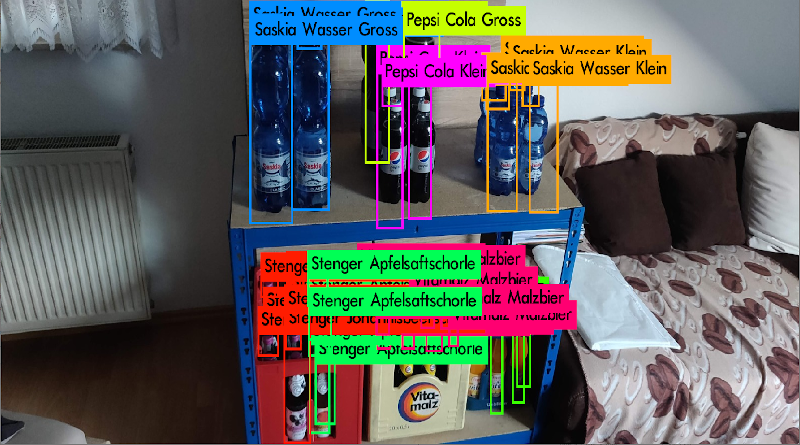
\includegraphics[width=13cm]{Bilder/yolo_inference.png} 
		\caption{Bildauszug aus Videostream nach der Inferenz mit YOLO}
		\label{yolo_inference}
	\end{center}
\end{figure}

Problem bei der Inferenz stellt nach wie vor die Detektion verdeckter Objekte dar. Beispielsweise sind Flaschen in Getränkekästen nur schwer detektierbar. Die Teilmerkmale verdeckter Objekte scheinen nicht ausreichend genug für eine zuversichtliche Detektion zu sein. Bei Herabsenken des \textit{confidence scores} zur Detektion gerade solcher Objekte werden wiederum zuvor doppelt detektierte Objekte erneut doppelt erkannt. Es lässt sich hierbei kein gutes Gleichgewicht einstellen. 

Die Inferenz findet nach der Definition im Konzeptionskapitel in Echtzeit statt. Allerdings besitzt das \textit{SmartWarehouse} Szenario ein weiteres zentrales Problem bei der Umsetzbarkeit. Dieses Problem beruht nicht auf technischer Natur, sondern auf der Auswahl des Verfahrens. Der Zählalgorithmus kann das selbe Objekt bei größeren zeitlichen Intervallen oder bei unterschiedlichen absoluten Positionen auf dem Bild nicht als das selbe Objekt identifizieren. Demnach werden Objekte in solchen Szenarien doppelt gezählt. Solange allerdings Objekte nur durch das Bild \glqq gleiten\grqq{} und nicht erneut nach einem gewissen Intervall im Bild zu finden sind, so lassen sich Objekte präzise zählen. Das Problem der doppelten Detektion lässt sich also nicht komplett mit dem Verfahren der Objektdetektion lösen, sondern nur auf konventionelle Verfahren mittels Scanning von Barcodes oder RFID-Chips. Das \textit{SmartWarehouse} Szenario ist somit nur unter bestimmten Umständen umsetzbar. 
